\documentclass[10pt]{article}
% \def\anonymous{1} before \documentclass gives the anonymous review version.
\ifdefined\anonymous \usepackage{tmlr} \else \usepackage[preprint]{tmlr} \fi
\usepackage{amsmath,amssymb,amsthm,booktabs,graphicx,microtype}
\usepackage{caption,url,xurl,xcolor}
\usepackage[section]{placeins}
\usepackage[colorlinks=true,allcolors=blue!55!black]{hyperref}
\captionsetup{font=small,labelfont=bf}
\setlength{\emergencystretch}{2em}

% Every number below comes from numbers.tex and tab_*.tex, which are written by
% pilot_neff/make_tables.py from result files. Do not type numbers by hand.
% main.tex compiles the clean paper; main_status.tex adds the working notes.
\newcommand{\ArchPerFamily}{116}
\newcommand{\ConsCoverHi}{90}
\newcommand{\ConsCoverLo}{57}
\newcommand{\DeclaredShare}{24}
\newcommand{\DifLlamaBases}{6}
\newcommand{\DifNamedFdrMax}{40}
\newcommand{\DifNamedFdrMin}{23}
\newcommand{\DifNamedMax}{48}
\newcommand{\DifNamedMin}{34}
\newcommand{\DifPermMax}{3}
\newcommand{\DifPermMin}{1}
\newcommand{\DifPermNoCCMax}{5}
\newcommand{\DifPermNoCCMin}{3}
\newcommand{\DifPlaceboMax}{9}
\newcommand{\DifPlaceboMin}{6}
\newcommand{\DifRepMax}{16}
\newcommand{\DifRepMin}{1}
\newcommand{\DifRepNullMax}{39}
\newcommand{\DifRepNullMin}{17}
\newcommand{\EffClusters}{10}
\newcommand{\FourthFamily}{49}
\newcommand{\GoldBenchmarks}{two benchmarks}
\newcommand{\GoldGsmAuroc}{0.73}
\newcommand{\GoldGsmBase}{9}
\newcommand{\GoldGsmFamAuroc}{0.69}
\newcommand{\GoldGsmFlagsFamily}{2}
\newcommand{\GoldGsmFlagsModel}{2}
\newcommand{\GoldGsmFlawed}{119}
\newcommand{\GoldGsmItems}{1,315}
\newcommand{\GoldGsmPrecFamily}{100}
\newcommand{\GoldGsmPrecModel}{100}
\newcommand{\GoldGsmTop}{44}
\newcommand{\GoldGsmWeightAuroc}{0.73}
\newcommand{\GoldMmluAligned}{5,602}
\newcommand{\GoldMmluAuroc}{0.55}
\newcommand{\GoldMmluBase}{6}
\newcommand{\GoldMmluDropped}{98}
\newcommand{\GoldMmluFamAuroc}{0.56}
\newcommand{\GoldMmluFlagsFamily}{475}
\newcommand{\GoldMmluFlagsModel}{658}
\newcommand{\GoldMmluFlawed}{364}
\newcommand{\GoldMmluItems}{5,602}
\newcommand{\GoldMmluPrecFamily}{11}
\newcommand{\GoldMmluPrecModel}{10}
\newcommand{\GoldMmluText}{MMLU-Redux \citep{gema2024mmlu} provides human annotations for 5,700 MMLU items; 5,602 of them could be matched unambiguously to the responses of the 842 archive models that were also evaluated on MMLU, and 364 of those are flawed. There the usual screen is much weaker (AUROC 0.55; 0.63 for the 105 items with a wrong answer key), and again no lineage-aware variant is distinguishable from it. Family-level testing reduces the significantly negative items from 658 to 475 without changing how many of them are documented as flawed (10\% and 11\%). }
\newcommand{\GoldMmluTop}{20}
\newcommand{\GoldMmluWeightAuroc}{0.54}
\newcommand{\GrowthCeiling}{12}
\newcommand{\GrowthDated}{914}
\newcommand{\GrowthFinalClusters}{7}
\newcommand{\GrowthPeak}{27}
\newcommand{\GrowthPeakEntries}{54}
\newcommand{\GrowthSettle}{130}
\newcommand{\IdentFalseEst}{5.6}
\newcommand{\IdentFalseTruth}{1.0}
\newcommand{\IdentMissEst}{1.0}
\newcommand{\IdentMissTruth}{2.1}
\newcommand{\InflARCTop}{24}
\newcommand{\InflGSMTop}{9}
\newcommand{\InflHellaSwagTop}{11}
\newcommand{\InflMedMax}{6.1}
\newcommand{\InflMedMin}{1.4}
\newcommand{\InflTruthfulQATop}{24}
\newcommand{\InflWinoGrandeTop}{35}
\newcommand{\LargestFamily}{332}
\newcommand{\LargestFamilyShare}{29}
\newcommand{\LayBalancedHi}{79}
\newcommand{\LayBalancedLo}{74}
\newcommand{\LayBootHi}{94}
\newcommand{\LayBootLo}{89}
\newcommand{\LayCuratedHi}{88}
\newcommand{\LayCuratedLo}{85}
\newcommand{\LayNewerHi}{42}
\newcommand{\LayNewerLo}{33}
\newcommand{\LineageCoverage}{84}
\newcommand{\LinkARC}{-0.04}
\newcommand{\LinkGSM}{+0.30}
\newcommand{\LinkHellaSwag}{-0.15}
\newcommand{\LinkTruthfulQA}{-0.06}
\newcommand{\LinkWinoGrande}{-0.38}
\newcommand{\NFamilies}{127}
\newcommand{\NModels}{1,151}
\newcommand{\ScreenLostMax}{52}
\newcommand{\ScreenLostMin}{16}
\newcommand{\ScreenSEMax}{2.0}
\newcommand{\ScreenSEMin}{1.4}
\newcommand{\ScreenVarMax}{4.1}
\newcommand{\ScreenVarMin}{1.9}
\newcommand{\SecondAssigned}{92}
\newcommand{\SecondClear}{14}
\newcommand{\SecondEffClusters}{25}
\newcommand{\SecondFamilies}{43}
\newcommand{\SecondFamily}{93}
\newcommand{\SecondInflMax}{1.3}
\newcommand{\SecondInflMin}{1.0}
\newcommand{\SecondLargest}{10}
\newcommand{\SecondPairs}{153}
\newcommand{\SecondTasks}{15}
\newcommand{\SimBootCoverHi}{90}
\newcommand{\SimBootCoverLo}{89}
\newcommand{\SimCRCoverHi}{93}
\newcommand{\SimCRCoverLo}{70}
\newcommand{\SimEffClusters}{10}
\newcommand{\SimFixDiffShared}{17.9}
\newcommand{\SimFixDiffUnrel}{19.4}
\newcommand{\SimItemRestMax}{6.8}
\newcommand{\SimItemRestMin}{1.7}
\newcommand{\SimNaiveCoverShared}{28}
\newcommand{\SimNaiveCoverUnrel}{37}
\newcommand{\SimNullNaive}{93}
\newcommand{\SimReps}{200}
\newcommand{\SimTCoverHi}{96}
\newcommand{\SimTCoverLo}{76}
\newcommand{\SimTrueDiffShared}{25.7}
\newcommand{\SimTrueDiffUnrel}{17.0}
\newcommand{\SimTrueDiscrShared}{6.5}
\newcommand{\SimTrueItemRestShared}{6.8}
\newcommand{\SimTrueItemRestUnrel}{1.7}
\newcommand{\SimUnevenCover}{37}
\newcommand{\SimUnevenEst}{3.3}
\newcommand{\SimUnevenFix}{3.0}
\newcommand{\ThinCoverHi}{94}
\newcommand{\ThinCoverLo}{93}
\newcommand{\ThinGainHi}{6.9}
\newcommand{\ThinGainLo}{4.5}
\newcommand{\ThirdFamily}{79}
\newcommand{\TransferRankAllSeeds}{3}
\newcommand{\UnassignedShare}{16}
\newcommand{\ValDeclared}{0.12}
\newcommand{\ValDifferent}{-0.02}
\newcommand{\ValSameFamily}{0.09}
\newcommand{\VfCoarse}{8}
\newcommand{\VfDirect}{76}
\newcommand{\VfEff}{14}
\newcommand{\VfFamilies}{368}
\newcommand{\VfImputed}{16}
\newcommand{\VfModels}{3,795}
\newcommand{\VfPerFamily}{273}
\newcommand{\VrAbove}{4}
\newcommand{\VrInflMax}{45}
\newcommand{\VrInflMin}{4}
\newcommand{\VrLostMax}{47}
\newcommand{\VrLostMin}{40}
\newcommand{\VrLostTasks}{3}
\newcommand{\VrModelsMax}{3,794}
\newcommand{\VrModelsMin}{1,822}
\newcommand{\VrNamedMax}{53}
\newcommand{\VrNamedMin}{17}
\newcommand{\VrPermMax}{4}
\newcommand{\VrPermMin}{2}
\newcommand{\VrPlaceboMax}{41}
\newcommand{\VrPlaceboMin}{12}
\newcommand{\VrRepMax}{38}
\newcommand{\VrRepMin}{1}
\newcommand{\VrRepNullMax}{59}
\newcommand{\VrRepNullMin}{15}
\newcommand{\VrSEMax}{4.5}
\newcommand{\VrSEMin}{2.6}
\newcommand{\VrSESplitMax}{2.4}
\newcommand{\VrSESplitMin}{1.6}
\newcommand{\VrSameAbove}{3}
\newcommand{\VrSameMax}{0.27}
\newcommand{\VrSameMin}{0.04}
\newcommand{\VrTasks}{4}
\newcommand{\VrTransferPos}{4}
\newcommand{\VtwoClusters}{15}
\newcommand{\VtwoClustersMax}{16}
\newcommand{\VtwoClustersMin}{12}
\newcommand{\VtwoFamilies}{428}
\newcommand{\VtwoLargestShare}{21}
\newcommand{\VtwoModels}{4,497}
\newcommand{\WeightGainHi}{7.5}
\newcommand{\WeightGainLo}{5.2}

\newif\ifdraft
\ifdefined\showstatus \drafttrue \else \draftfalse \fi
\newcommand{\todo}[1]{\ifdraft\textcolor{blue!70!black}{[TODO: #1]}\fi}
\newtheorem{proposition}{Proposition}
\newtheorem{corollary}{Corollary}
\theoremstyle{remark}\newtheorem{remark}{Remark}
\DeclareMathOperator{\Var}{Var}
\DeclareMathOperator{\Cov}{Cov}
\DeclareMathOperator{\tr}{tr}
\newcommand{\deff}{\mathrm{deff}}

\title{Count Lineages, Not Checkpoints:\\LLMs Are Not Independent Test-Takers}
\author{\name Pavan Reddy Mogili}
\date{}

\begin{document}
\maketitle

\begin{abstract}
Item-level analyses of language-model benchmarks, such as item response
models, label-error screens, and differential item functioning, are usually
run as if every evaluated model were an independent respondent. Leaderboard
panels are not like that: most entries share a base model with many others. We
work out what this does to uncertainty and how to repair it.
We take lineage from repository metadata and not from responses, because a
family of related models and an extra ability dimension are observationally
equivalent in a response matrix. Of \NModels{} archived Open LLM Leaderboard
entries, \LineageCoverage\% can be assigned to a base-model family and
\LargestFamilyShare\% belong to a single one; by family sizes the panel is as
concentrated as about \EffClusters{} equal families, and its
\VtwoModels-entry successor as about \VtwoClusters. Models that share only a
base model answer nearly as alike as declared relatives.
The resulting variance inflation depends on the statistic, so no single
``effective number of models'' exists; we derive it for item difficulty,
discrimination, and inter-item association. In a simulation matched to the
archive's family sizes and within-family similarity, nominal 95\% intervals for
item difficulty cover their target
\SimNaiveCoverShared--\SimNaiveCoverUnrel\% of the time. Resampling whole
families restores \SimBootCoverLo--\SimBootCoverHi\%, and weighting families
equally lowers the variance of difficulty estimates
\WeightGainLo--\WeightGainHi-fold.
On the archive's real responses, family-level standard errors of item--rest
correlations are \ScreenSEMin--\ScreenSEMax{} times model-level ones, and
\ScreenLostMin--\ScreenLostMax\% of the items a screen flags as significantly
negative lose significance. Under a standard test for differential item
functioning, two arbitrary collections of unrelated base models differ on
\VrPlaceboMin--\VrPlaceboMax\% of items on a newer leaderboard, so claims
about named families need a lineage baseline. Against documented label
errors, lineage-aware scores rank flawed items no better than the usual
screen: lineage changes how much evidence a flag carries, not which items to
inspect first. We release family labels and a small tool.
\end{abstract}

\section{Introduction}
Comparative biology learned in the 1980s that species are not independent data
points: closely related species share traits by descent, so treating them as
separate observations overstates the evidence for any cross-species pattern
\citep{felsenstein1985phylogenies}. Item-level evaluation of language models is
in the same position. A response matrix records which of $M$ models answered
which of $J$ benchmark questions correctly. The standard errors and tests used
with item response theory, label-error screens, benchmark compression, and
differential item functioning are derived for $M$ respondents drawn
independently from a population
\citep{polo2024tinybenchmarks,kipnis2025metabench,truong2025fantastic,land2026auditing,dif2026llm}.
The respondents are not independent. Public leaderboards consist largely of
derivatives of a small number of base models, and even curated panels contain
several releases of the same model line.

The concern is recognised, and existing remedies work on responses or names.
\citet{truong2025fantastic} note that shared training data can shrink the
effective sample size, and examine sensitivity to the composition of the model
pool by creator, size, and release date. \citet{land2026auditing} drop models
whose response vectors are nearly identical and state that, among the 114 that
remain, ``the effective number of independent respondents remains below 114,''
leaving the number open. \citet{neartied2026rankings} split models by owner
and thin to one checkpoint per owner and named family. Model similarity itself
has been measured: errors are correlated across models and more so among
stronger ones \citep{kim2025correlated,goel2025great}, and benchmark
prediction depends on how similar target models are to source models
\citep{zhang2025benchmarkprediction}. What is missing is the step from
``models are similar'' to ``this standard error is too small by this factor,''
together with a way to obtain that factor that can be trusted. This paper
supplies both, and shows why estimating the dependence from the responses
themselves is unreliable.

\paragraph{Contributions.}
\begin{enumerate}\itemsep2pt
\item \textbf{Variance inflation is statistic-specific
  (\S\ref{sec:theory}).} For a linear item statistic the inflation is a
  quadratic form in the model--model residual correlation matrix along the
  statistic's weight vector; for an association between items it is governed by
  the sum of \emph{squared} correlations. A single effective sample size
  therefore misstates uncertainty for most statistics.
\item \textbf{Responses alone do not identify the dependence
  (\S\ref{sec:ident}).} A family random-effects model is a multidimensional
  response model whose extra person coordinates are family indicators; the two
  differ only in which quantities are resampled. In simulation, grouping models
  by response similarity fails in both directions.
\item \textbf{Lineage from outside the responses (\S\ref{sec:lineage}).}
  Declared parent chains, configuration signatures, and repository names
  recover a base-model family for \LineageCoverage\% of a \NModels-entry
  archive. The labels never see a benchmark response, and they predict
  response similarity on that archive, on a curated panel, and on a newer
  leaderboard.
\item \textbf{Size of the problem and working corrections
  (\S\ref{sec:size}).} With the archive's family layout and its observed
  within-family similarity, intervals that ignore lineage are badly
  miscalibrated for difficulty and, when relatives share ability, for
  discrimination and item--rest correlation as well. A bootstrap over whole
  families restores most of the coverage, and weighting families equally
  recovers precision that the unweighted panel throws away.
\item \textbf{Re-audits of two procedures (\S\ref{sec:screens}).} Against a
  model-level bootstrap, family-level testing removes
  \ScreenLostMin--\ScreenLostMax\% of the items a screen flags as significantly
  negative. Under a standard test
  for differential item functioning, arbitrary collections of unrelated base
  models already differ on many items, and effects found for a named family
  are mostly specific to individual base models. Against documented label
  errors, lineage-aware scores do not rank flawed items better than the usual
  screen.
\end{enumerate}

We do not propose a new psychometric model or a new error detector.
Cluster-robust inference
\citep{liang1986longitudinal,cameron2015practitioner,mackinnon2023cluster},
design effects \citep{kish1965survey}, and blocked validation
\citep{roberts2017crossvalidation} are established. The contribution is to
work out what they imply for item-level evaluation of language models, to show
why the cluster labels should come from lineage and not from behaviour, and to
measure the consequences on public data.

\section{Related work}\label{sec:related}
\paragraph{Item-level evaluation.}
IRT-based analysis and compression of LLM benchmarks
\citep{lalor2016irt,rodriguez2021informative,polo2024tinybenchmarks,kipnis2025metabench,hofmann2025fluid,zhou2026lost},
label-error screening \citep{northcutt2021labelerrors,gema2024mmlu,truong2025fantastic,land2026auditing},
option-level models \citep{fei2026everywrong}, and reliability of IRT
estimation \citep{jiang2026trustirt} all condition on a panel of models. To
our knowledge none reports item-level uncertainty with lineage as the sampling
unit.

\paragraph{Model families in item-level analysis.}
Two concurrent studies are closest. \citet{dif2026llm} apply Mantel--Haenszel
differential item functioning to Llama and Qwen models on six benchmarks and
find many items that favour one family at equal total score.
\citet{neartied2026rankings} estimate residual item-by-family effects after a
multidimensional adjustment, on five benchmarks drawn from RouterEval
\citep{huang2025routereval}, and show that near-tied cross-family rankings can
reverse when low-DIF items are selected. They assign families by model name,
split by model owner, cap each owner--family pair at five checkpoints, and
rank one representative per pair. Both treat item-by-family effects as fixed
quantities to be estimated and ask what they do to scores and rankings. We
treat the same effects as a source of sampling dependence and ask what they do
to the uncertainty of item statistics; Proposition~\ref{prop:equiv} makes the
relation between the two views exact.
\todo{We read the method of \citet{neartied2026rankings} in full but only the abstract of \citet{dif2026llm}; read the latter in full before submission.}

\paragraph{Model similarity and lineage.}
\citet{yax2025phylolm} reconstruct model phylogenies from outputs and hold out
whole families when predicting benchmark scores. \citet{kim2025correlated} and
\citet{goel2025great} measure correlated errors across more than a hundred
models each. \citet{zhang2025benchmarkprediction} show that benchmark
prediction depends on model similarity and degrades when extrapolating to
stronger models. \citet{laufer2025anatomy} and \citet{horwitz2025atlas} build
lineage graphs of public models from repository metadata.
\citet{kohli2026nine} computes an effective number of votes for panels of
correlated LLM judges. We use metadata lineage for a different purpose: as the
sampling unit for item statistics.

\paragraph{Dependent observations.}
Design effects \citep{kish1965survey}, cluster-robust variance and its
small-cluster corrections
\citep{liang1986longitudinal,cameron2015practitioner,carter2017asymptotic,mackinnon2023cluster},
effective degrees of freedom for second-moment statistics
\citep{bretherton1999effective}, blocked validation
\citep{roberts2017crossvalidation}, phylogenetic comparative methods
\citep{felsenstein1985phylogenies}, and duplicate leakage
\citep{allamanis2019duplication,kapoor2022leakage} supply the statistical
tools. \citet{miller2024errorbars} cluster \emph{questions} when comparing
models; we cluster \emph{models} when studying questions.

\section{Setting and estimands}\label{sec:setup}
Let $X\in\{0,1\}^{M\times J}$ be a complete response matrix. Each item $j$ has
a response function $P_{ij}=\Pr(X_{ij}=1)$ that depends on a scalar ability
proxy $z_i$, the logit of model $i$'s accuracy standardised within the panel.
We study four statistics per item: difficulty (the logistic intercept, that is,
the log-odds of a correct answer at the panel's mean ability), discrimination
(the logistic slope on $z$), the item--rest correlation used by screening
methods, and the residual association between two items after removing
ability.

Uncertainty is defined with respect to a sampling model for \emph{models}. The
naive model draws the $M$ rows independently. The lineage model draws
\emph{families} independently and lets models within a family share
item-level deviations. The \emph{variance inflation} (design effect) of a
statistic is the ratio of its variance under the lineage model to its variance
under independence with the same marginal response functions. Which model is
appropriate is a statement about the target population, taken up in
\S\ref{sec:ident}.

\section{Variance inflation depends on the statistic}\label{sec:theory}
Fix an item $j$ and let $e_j\in\mathbb R^M$ be its residuals across models
under the sampling model, with mean zero, unit variances, and
$\Cov(e_j)=R$, a correlation matrix with entries $\rho_{ik}$. Independence
corresponds to $R=I$.

\begin{proposition}[Linear statistics]\label{prop:linear}
For $T=w^\top e_j$ with fixed weights $w$,
$\deff(w)=w^\top R\,w/w^\top w$. For equal weights ($w\propto\mathbf 1$, the
item mean) this is $1+M^{-1}\sum_{i\ne k}\rho_{ik}$; for weights proportional
to centred ability ($w\propto z-\bar z$) it is the same quadratic form along
the ability direction.
\end{proposition}
\noindent\emph{Proof.} $\Var(w^\top e_j)=w^\top R\,w$, and under independence
$R=I$. \qed

\begin{proposition}[Association statistics]\label{prop:assoc}
For items $j\neq l$ whose residual vectors are independent of each other,
each with mean zero and covariance $R$,
$\Var(e_j^\top e_l)=\tr(R^2)$, so
$\deff_{\mathrm{assoc}}=1+M^{-1}\sum_{i\ne k}\rho_{ik}^2$.
\end{proposition}
\noindent\emph{Proof.} The cross-product has mean zero, and
$\mathbb E[(e_j^\top e_l)^2]=\mathbb E[e_j^\top(e_le_l^\top)e_j]
=\mathbb E[e_j^\top R\,e_j]=\tr(R^2)=M+\sum_{i\ne k}\rho_{ik}^2$; under
independence $\tr(I)=M$. \qed

\begin{corollary}[Families]\label{cor:families}
If models fall into families of sizes $m_g$ with within-family correlation
$\rho_g\in[0,1]$ and no correlation across families, then
\[
\deff_{\mathrm{mean}}=1+\frac1M\sum_g m_g(m_g-1)\rho_g,\qquad
\deff_{\mathrm{assoc}}=1+\frac1M\sum_g m_g(m_g-1)\rho_g^2
\le\deff_{\mathrm{mean}} .
\]
With $\rho_g=1$ both reduce to Kish's $M^{-1}\sum_g m_g^2$
\citep{kish1965survey}. For fixed abilities the slope-type inflation is
$1+\sum_g\rho_g\sum_{i\ne k\in g}\tilde z_i\tilde z_k/\sum_i\tilde z_i^2$ with
$\tilde z=z-\bar z$: equal to one on average when relatives have unrelated
abilities, and large when relatives share ability.
\end{corollary}

Logistic difficulty and discrimination are not exactly linear statistics: they
are asymptotically linear in the residuals with item-specific weights, and
they are estimated on an ability scale that is itself computed from the panel.
The propositions therefore describe the mechanism; \S\ref{sec:calib} measures
the estimators as they are used.

Three consequences follow. A panel has no single effective size. Inflation is
linear in $\rho$ for the item mean, so relatedness too weak to see in any
pairwise comparison still matters: with $\rho_g=0.1$ in a family of 300, that
family alone contributes $0.1\times 300\times 299/M$. And the layout enters
through $\sum_g m_g^2$. We call $G^\ast=M^2/\sum_g m_g^2$ the
\emph{effective number of families}: the number of equal-sized families with
the same concentration. It is the Kish effective sample size only in the
limit $\rho_g=1$, and a simplification of the effective number of clusters of
\citet{carter2017asymptotic}; we use it as a description of the panel, not as
a count of independent models.

\begin{remark}[In-sample degeneracy]\label{rem:degenerate}
The score equations of a fitted item response function make each item's
residuals sum to zero across models and be orthogonal to ability. Summing or
ability-weighting an estimated residual correlation matrix over \emph{all}
pairs therefore returns approximately zero, whatever the dependence. The
inflation of difficulty and discrimination can be estimated only by
restricting to pairs that a cluster structure declares related, which is why
cluster-robust estimators need the family labels as an input.
\end{remark}

\section{Responses alone do not identify the dependence}\label{sec:ident}
Fix item parameters $(a_j,b_j)$ and a partition $g$ of the models into $G$
groups, and consider two sampling models for a panel.
\begin{itemize}\itemsep1pt
\item[\textbf{F}] \emph{Families are sampled.} Each group $g$ draws item
  effects $u_{g\cdot}\in\mathbb R^J$ independently from a distribution $Q$;
  each member draws $\theta_i$ independently; responses are independent
  Bernoulli with $\operatorname{logit}P_{ij}=a_j(\theta_i-b_j)+u_{g(i)j}$.
\item[\textbf{D}] \emph{Profiles are fixed.} There are $G$ fixed profiles with
  loadings $C\in\mathbb R^{G\times J}$; model $i$ has profile $g(i)$ and draws
  $\theta_i$ independently; responses are independent Bernoulli with
  $\operatorname{logit}P_{ij}=a_j(\theta_i-b_j)+C_{g(i)j}$. This is a
  multidimensional response model whose extra person coordinates are profile
  indicators.
\end{itemize}

\begin{proposition}[Observational equivalence]\label{prop:equiv}
(i) The law of the response matrix under F is the mixture, over $u\sim Q^{G}$,
of its laws under D with $C=u$. Consequently any test of ``D holds for some
$C$'' that has level $\alpha$ for every $C$ has power at most $\alpha$ against
F: a single response matrix cannot show that item-by-group effects are
resampled with the groups and not fixed features of the population.
(ii) Under D the rows of $X$ are independent given $C$, so an item mean has
its independent-sampling variance. Under F, for the item mean $\hat p_j$,
$\Var(\hat p_j)\ge\Var\big(\mathbb E[\hat p_j\mid u]\big)
=M^{-2}\sum_g m_g^2\Var(\mu_{gj})$ with
$\mu_{gj}=\mathbb E[X_{ij}\mid u_{gj}]$, a term proportional to $1/G^\ast$
that does not vanish as $M$ grows unless $G^\ast$ grows too.
\end{proposition}
\noindent\emph{Proof.} (i) Conditional on $u$, model F is model D with $C=u$,
so the F law is the stated mixture; a test with level $\alpha$ under every
component has rejection probability at most $\alpha$ under the mixture.
(ii) Under D the rows are independent given the fixed $C$. Under F the law of
total variance gives the bound, and
$\mathbb E[\hat p_j\mid u]=M^{-1}\sum_g m_g\mu_{gj}$ with the $\mu_{gj}$
independent across groups. \qed

The two models describe different target populations. D asks how these
particular base models respond; F asks about model lineages in general, of
which the observed base models are a sample. The data cannot choose between
them, so the analyst must. Differential item functioning across named
families \citep{dif2026llm,neartied2026rankings} adopts the fixed view of the
same structure: its item-by-family effects are our $u$.

A second obstacle is that the groups themselves are not observed. For an
unnormalised residual matrix $E$,
$\tr\big((EE^\top)^2\big)=\tr\big((E^\top E)^2\big)$: the total squared
similarity between models equals the total squared association between items.
A low-rank component of $E$ is simultaneously ``some models behave alike'' and
``some items measure something extra,'' so similarity in responses does not by
itself indicate lineage.

\paragraph{Simulation.}
Table~\ref{tab:ident} shows what this means for one natural response-only
approach. We simulate 300 models and 800 items under a two-parameter logistic
model, with families of sizes 40, 25, 15, two of 10, eight of 5, twenty of 2,
and 120 singletons. True inflation is the median over items of the Monte Carlo
variance ratio against an independent panel. We compare it with (i) the
expressions of Corollary~\ref{cor:families} evaluated with the true family
labels and (ii) two response-only estimators: cluster-robust variance with
groups found by average-linkage clustering of residual correlations at a
threshold of 0.35, and the sum over all model pairs of the product of residual
correlations computed on two disjoint halves of the items.
\begin{table}[!htb]\centering\small
\caption{Can dependence be read from responses? Simulated panels of 300 models and 800 items (100 replicates). True inflation is the median over items of the Monte Carlo variance ratio against an independent panel. With the true family labels the expressions of Corollary~\ref{cor:families} are close to the truth whenever families are present (A, B, E). The response-only estimators miss weak families entirely (B), understate difficulty inflation for strong ones (A, E), and report inflation among independent models that differ on a second ability dimension (C, D).}\label{tab:ident}
\begin{tabular}{lrr|rr|rr}
\toprule
 & \multicolumn{2}{c|}{True inflation} & \multicolumn{2}{c|}{True labels} & \multicolumn{2}{c}{Response-only}\\
Scenario & difficulty & assoc. & difficulty & assoc. & difficulty & assoc.\\
\midrule
A\; strong families & 4.02 & 1.91 & 3.89 & 1.92 & 1.50 & 2.13\\
B\; weak families & 2.12 & 1.14 & 2.12 & 1.14 & 1.00 & 1.18\\
C\; second dimension only & 1.00 & 0.99 & 0.97 & 1.05 & 1.02 & 2.61\\
D\; strong second dimension & 0.97 & 0.98 & 0.98 & 1.34 & 5.60 & 12.16\\
E\; families + second dimension & 3.71 & 1.83 & 3.67 & 1.81 & 1.40 & 2.39\\
\bottomrule
\end{tabular}
\end{table}

Given the true labels, the expressions track difficulty and association when
families are present. Without labels, weak families go undetected (true
difficulty inflation \IdentMissTruth$\times$, estimate
\IdentMissEst$\times$), and a strong second ability dimension among
independent models is reported as \IdentFalseEst$\times$ inflation when the
truth is \IdentFalseTruth$\times$. A lower clustering threshold would trade
one error for the other. Any study that groups models by behavioural
similarity and treats the groups as lineages inherits this trade-off.

\section{Lineage from outside the responses}\label{sec:lineage}
\paragraph{Archive.} We use \NModels{} model entries from the Open LLM
Leaderboard archive \citep{openllmleaderboard}, evaluated with the
\texttt{lm-evaluation-harness} \citep{eval-harness} on ARC-Challenge,
HellaSwag, TruthfulQA, WinoGrande, and GSM8K
\citep{clark2018arc,zellers2019hellaswag,lin2022truthfulqa,sakaguchi2021winogrande,cobbe2021gsm8k}.
Items answered identically by every model are dropped, and each benchmark uses
the entries with complete responses.

\paragraph{Recovery.} For every entry we query public Hugging Face repository
metadata and use three signals, none of which involves a benchmark response:
(i) declared parents, from the model card's base-model field and adapter
configuration, followed for up to four hops; (ii) a configuration signature,
namely architecture class, hidden size, layer count, and, where several base
models share that shape, feed-forward width and vocabulary size;
(iii) tokens in the repository name. A model is assigned to a
\emph{base-model family} by signature when its configuration is readable,
otherwise by the signature or name of its declared root, otherwise by its own
name.
\begin{table}[!htb]\centering\small
\caption{Lineage recovery for the 1,151-entry archive from public repository metadata retrieved on 15 November 2026.}\label{tab:coverage}
\begin{tabular}{lrr}
\toprule
Signal & Entries & Share\\
\midrule
Repository still public & 914 & 79\%\\
Configuration readable & 865 & 75\%\\
Declares a parent model & 274 & 24\%\\
\midrule
Family assigned by configuration signature & 856 & 74\%\\
Family assigned by declared root & 36 & 3\%\\
Family assigned by repository name only & 72 & 6\%\\
\textbf{Family assigned, any signal} & \textbf{964} & \textbf{84\%}\\
Unassigned (treated as singletons) & 187 & 16\%\\
\bottomrule
\end{tabular}
\end{table}


Fine-grained lineage is sparse: only \DeclaredShare\% of entries declare a
parent. Family membership is not: \LineageCoverage\% can be assigned
(Table~\ref{tab:coverage}). The panel is concentrated. \LargestFamily{}
entries (\LargestFamilyShare\%) are assigned to the Mistral-7B family; the
next three families have \SecondFamily, \ThirdFamily, and \FourthFamily{}
entries, and there are \NFamilies{} labelled families in all, giving
$G^\ast\approx\EffClusters$.

\begin{figure}[!htb]\centering
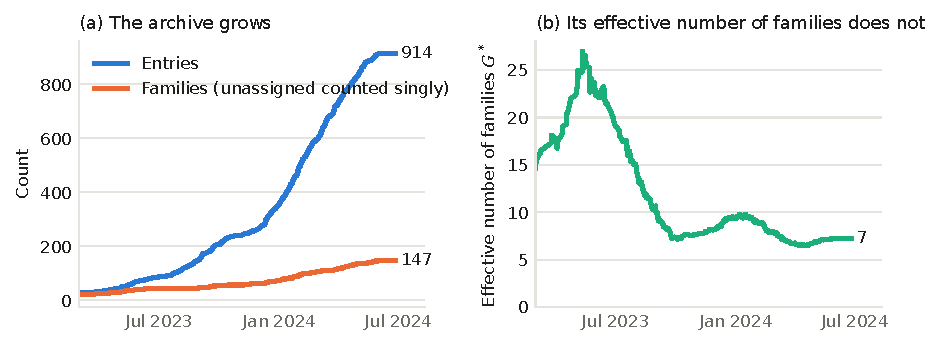
\includegraphics[width=\linewidth]{figures/f3_growth.pdf}
\caption{The \GrowthDated{} archive entries whose repository creation date is
known, in order of creation; the axis starts in March 2023, by which date the
earliest repositories are already counted. (a) Entries and families, with
each unassigned entry counted as its own family. (b) Effective number of
families $G^\ast=M^2/\sum_g m_g^2$.}
\label{fig:growth}
\end{figure}

More entries did not mean more effective families. Ordering the
\GrowthDated{} entries with a known repository creation date,
$G^\ast$ peaks at about \GrowthPeak{} after \GrowthPeakEntries{} entries, a
stage dominated by base models that predate the leaderboard, and has stayed
below \GrowthCeiling{} since about \GrowthSettle{} entries while the count
grew to \GrowthDated{} (Figure~\ref{fig:growth}). New families kept arriving,
but derivatives of a few base models arrived as fast. Creation dates stand in
for submission order and are missing for deleted repositories, most of which
are unassigned, which is why $G^\ast$ for the dated subset
(\GrowthFinalClusters) is below the full archive's.

\paragraph{A newer leaderboard.}
The successor leaderboard \citep{fourrier2024leaderboardv2} ran from June 2024
to March 2025 and recorded architecture and parameter count for each of its
\VtwoModels{} entries. With families defined from those two fields, it has
\VtwoFamilies{} families, the largest holding \VtwoLargestShare\% of entries,
and $G^\ast\approx\VtwoClusters$; $G^\ast$ stayed between \VtwoClustersMin{}
and \VtwoClustersMax{} from its first thousand entries onward. This
definition is coarser than the archive's, but for the \VfModels{} entries
whose responses we analyse in \S\ref{sec:newer}, the archive's
configuration-based definition gives nearly the same value
($G^\ast\approx\VfEff$).
Table~\ref{tab:panels} sets three panels side by side: over a thousand and
several thousand entries are as concentrated as ten to fifteen equal
families, and a curated panel of 100 is less concentrated than either.
\begin{table}[!htb]\centering\small
\caption{Lineage composition of three panels. Families count unassigned entries as singletons. $G^\ast$ is the effective number of families. For the newer leaderboard, families are defined from the architecture and parameter count recorded at submission, which is coarser than the configuration signature used for the other two panels.}\label{tab:panels}
\resizebox{\linewidth}{!}{%
\begin{tabular}{llrrrr}
\toprule
Panel & Period & Entries & Families & Largest family & $G^\ast$\\
\midrule
Open LLM Leaderboard archive & 2023--mid 2024 & 1,151 & 314 & 29\% & 10\\
Newer Open LLM Leaderboard, all entries & June 2024--March 2025 & 4,497 & 428 & 21\% & 15\\
BenchMIRT (curated subset of the newer one) & to early 2025 & 100 & 51 & 10\% & 25\\
\bottomrule
\end{tabular}}
\end{table}


\begin{figure}[!htb]\centering
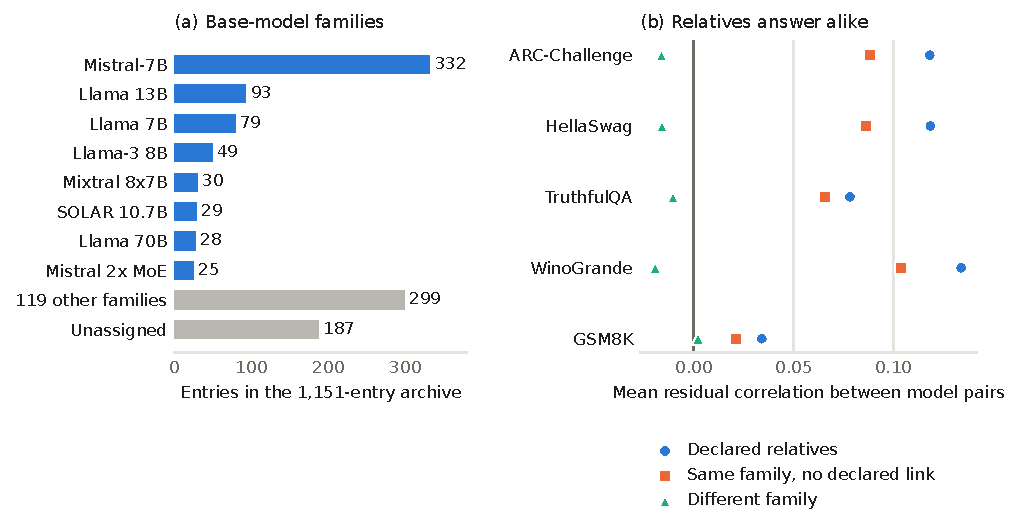
\includegraphics[width=\linewidth]{figures/f1_lineage.pdf}
\caption{(a) Base-model families in the archive, from repository metadata.
(b) Mean ability-adjusted residual correlation between pairs of models. Models
that share a base model answer alike whether or not a link is declared; models
from different families do not. Values are in Table~\ref{tab:validation}.}
\label{fig:lineage}
\end{figure}

\paragraph{Validation against responses.}
The labels were built without responses, so their relation to response
similarity is a test and not a tautology (Figure~\ref{fig:lineage},
Table~\ref{tab:validation}).
\begin{table}[!htb]\centering\small
\caption{Mean ability-adjusted residual correlation between pairs of models, by lineage relation. Labels were built without any benchmark response. Declared relatives: connected through declared parent links. Same family: same base-model family but no declared link. Different family: different families and no declared link.}\label{tab:validation}
\begin{tabular}{lrrr}
\toprule
Benchmark & Declared relatives & Same family, no declared link & Different family\\
\midrule
ARC-Challenge & $+0.118$ & $+0.088$ & $-0.016$\\
HellaSwag & $+0.118$ & $+0.086$ & $-0.016$\\
TruthfulQA & $+0.078$ & $+0.066$ & $-0.010$\\
WinoGrande & $+0.134$ & $+0.104$ & $-0.019$\\
GSM8K & $+0.034$ & $+0.021$ & $+0.002$\\
\bottomrule
\end{tabular}
\end{table}

Models that share only a base model are almost as alike as declared relatives.
Relatedness is therefore much more widespread than model cards document, and
the pairwise correlations involved, around 0.1, are the weak and widespread
kind that Corollary~\ref{cor:families} says matters for difficulty and that
threshold-based grouping of responses does not see (Table~\ref{tab:ident},
scenario B).

\section{How large is the problem?}\label{sec:size}
\subsection{A simulation matched to the archive}\label{sec:calib}
The true inflation on real data is unknown, so we first measure it in a
simulation that copies the archive's family layout exactly (\NModels{} models,
the same family sizes) and sets the spread of family-by-item effects so that
the mean within-family residual correlation falls within the range observed in
Table~\ref{tab:validation}. We vary whether relatives share ability (half of
the ability variance common to the family) and whether family effects are
concentrated in a subset of items. True inflation is the median over items of
the Monte Carlo variance ratio against a panel of independent models with the
same marginals. Because ability is standardised within each panel, the point
at which difficulty is measured moves when a large family's ability moves; we
therefore also report the inflation with the ability scale held fixed across
replicates.
\begin{table}[!htb]\centering\footnotesize\setlength{\tabcolsep}{3.5pt}
\caption{True variance inflation for the median item on the archive's family layout (1,151 models; 400 items; 200 replicates; family-effect spread 1.1 on the logit scale), and estimates that use the true family labels. $\bar r$ is the mean within-family residual correlation, for comparison with Table~\ref{tab:validation}. ``Fixed'' holds the ability scale fixed across replicates. The cluster-jackknife estimates of difficulty inflation run below the truth when one family dominates.}\label{tab:simtruth}
\resizebox{\linewidth}{!}{%
\begin{tabular}{lr|rrrrrr|rrr}
\toprule
 & & \multicolumn{6}{c|}{True inflation} & \multicolumn{3}{c}{Estimated, true labels}\\
Scenario & $\bar r$ & diff. & fixed & discr. & fixed & item--rest & assoc. & diff. & discr. & assoc.\\
\midrule
No families & 0.00 & 1.0 & 1.0 & 1.0 & 1.0 & 1.0 & 1.0 & 0.9 & 1.0 & 1.0\\
Families, unrelated ability & 0.11 & 17.0 & 19.4 & 1.5 & 1.5 & 1.7 & 2.8 & 11.9 & 1.2 & 2.4\\
Families, shared ability & 0.09 & 25.7 & 17.9 & 6.5 & 5.7 & 6.8 & 2.6 & 12.5 & 4.2 & 2.2\\
Shared ability, uneven items & 0.07 & 11.9 & 3.0 & 2.2 & 1.6 & 2.7 & 1.2 & 3.3 & 1.7 & 1.7\\
\bottomrule
\end{tabular}}
\end{table}

\begin{table}[!htb]\centering\footnotesize\setlength{\tabcolsep}{3.5pt}
\caption{Share (\%) of nominal 95\% intervals that contain the Monte Carlo mean of the estimator, in the same simulation; this measures the calibration of the standard error. Naive: model-based standard errors treating models as independent. CR0: cluster-robust with families as clusters. CR3: linearised delete-one-family jackknife with a normal critical value. CR3+$t$: CR3 with a $t$ critical value on $G^\ast-1$ degrees of freedom. Bootstrap: percentile interval from resampling whole families (40 replicates, 99 resamples, 120 items). Monte Carlo standard errors are at most 1.4 points for the first four methods and 1.8 for the bootstrap.}\label{tab:simcover}
\begin{tabular}{l|rrrrr|rrrr}
\toprule
 & \multicolumn{5}{c|}{Difficulty} & \multicolumn{4}{c}{Discrimination}\\
Scenario & naive & CR0 & CR3 & CR3+$t$ & boot. & naive & CR3 & CR3+$t$ & boot.\\
\midrule
No families & 93 & 90 & 92 & 95 & 92 & 94 & 93 & 96 & 92\\
Families, unrelated ability & 35 & 86 & 93 & 96 & 90 & 89 & 92 & 95 & 92\\
Families, shared ability & 28 & 71 & 83 & 87 & 90 & 60 & 90 & 94 & 91\\
Shared ability, uneven items & 37 & 61 & 70 & 76 & 89 & 73 & 89 & 93 & 93\\
\bottomrule
\end{tabular}
\end{table}

\begin{figure}[!htb]\centering
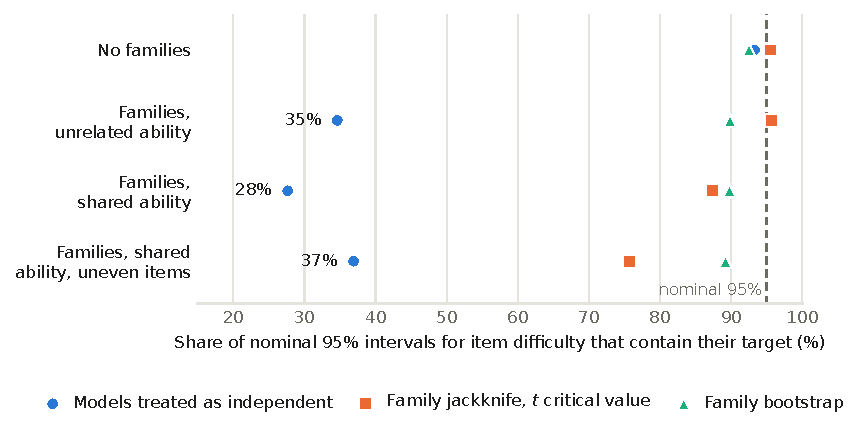
\includegraphics[width=0.8\linewidth]{figures/f2_coverage.pdf}
\caption{Share of nominal 95\% intervals for item difficulty that contain
their target, in a simulation with the archive's family layout and
within-family similarity. The cluster jackknife uses the $t$ critical value of
Table~\ref{tab:simcover}. Values are in that table.}
\label{fig:coverage}
\end{figure}

Table~\ref{tab:simtruth} shows the statistic-specific pattern predicted by
Corollary~\ref{cor:families}. With unrelated abilities, the variance of the
median item's difficulty is inflated \SimTrueDiffUnrel-fold while its
item--rest correlation is inflated \SimTrueItemRestUnrel-fold. When relatives
share ability, discrimination and the item--rest correlation are inflated too
(\SimTrueDiscrShared$\times$ and \SimTrueItemRestShared$\times$), and
difficulty inflation rises to \SimTrueDiffShared$\times$. That rise is the
moving reference point: with the ability scale held fixed, difficulty
inflation is \SimFixDiffUnrel$\times$ and \SimFixDiffShared$\times$ in the two
scenarios, and when family effects are concentrated in a minority of items the
median item's fixed-scale inflation is \SimUnevenFix$\times$. None of these is an effective sample size for the panel; they are
properties of one statistic for a typical item.

Table~\ref{tab:simcover} and Figure~\ref{fig:coverage} give the practical
consequence. The table reports how often a nominal 95\% interval contains the
long-run mean of the estimator, which isolates the calibration of the standard
error. Intervals that treat models as independent do so in
\SimNaiveCoverShared--\SimNaiveCoverUnrel\% of cases for difficulty, against
\SimNullNaive\% when there are no families, the shortfall from 95\% in that
case reflecting ability being an estimated proxy. Clustering on the true
families helps. The cluster jackknife recommended for unbalanced clusters
\citep{mackinnon2023cluster} reaches \SimCRCoverLo--\SimCRCoverHi\%; replacing
its normal critical value by a $t$ value on $G^\ast-1$ degrees of freedom, a
heuristic of ours, gives \SimTCoverLo--\SimTCoverHi\%, accurate when
relatives have unrelated abilities and short when they share ability, because
the jackknife conditions on the estimated ability scale. A bootstrap that
resamples whole families and recomputes ability reaches
\SimBootCoverLo--\SimBootCoverHi\% in every family scenario. Neither is exact
with $G^\ast\approx\SimEffClusters$, and the jackknife's estimated inflation
is below the truth for difficulty (Table~\ref{tab:simtruth}, right); both are
far closer than the naive analysis.

\paragraph{Other family layouts.}
How bad the naive analysis is depends on how concentrated the panel is
(Table~\ref{tab:simlayouts}). With the newer leaderboard's family sizes,
naive intervals for difficulty cover \LayNewerLo--\LayNewerHi\%, much as on
the archive layout. With the same number of models spread over 115 families
of ten they cover \LayBalancedLo--\LayBalancedHi\%, and with the curated
panel's sizes \LayCuratedLo--\LayCuratedHi\%. Across all four layouts and
all family scenarios the family bootstrap covers
\LayBootLo--\LayBootHi\%.
\begin{table}[!htb]\centering\footnotesize\setlength{\tabcolsep}{3.5pt}
\caption{The matched simulation under four family layouts (400 items; 200 replicates for the archive layout, 300 for the curated panel, 120 otherwise). The newer leaderboard's family sizes are scaled to the archive's panel size. $G^\ast$: effective number of families. True inflation of difficulty for the median item on the panel's own ability scale and on a fixed scale, and of the item--rest correlation. Coverage (\%) of nominal 95\% intervals for difficulty: naive, family jackknife with a $t$ critical value, and family bootstrap.}\label{tab:simlayouts}
\begin{tabular}{lrrlr|rrr|rrr}
\toprule
 & & & & & \multicolumn{3}{c|}{True inflation} & \multicolumn{3}{c}{Coverage (\%)}\\
Layout & $M$ & $G^\ast$ & Scenario & $\bar r$ & diff. & fixed & item--rest & naive & CR3+$t$ & boot.\\
\midrule
Archive & 1,151 & 10 & Unrelated ability & 0.11 & 17.0 & 19.4 & 1.7 & 35 & 96 & 90\\
 & &  & Shared ability & 0.09 & 25.7 & 17.9 & 6.8 & 28 & 87 & 90\\
 & &  & Shared, uneven items & 0.07 & 11.9 & 3.0 & 2.7 & 37 & 76 & 89\\
\midrule
Newer leaderboard, scaled & 1,151 & 14 & Unrelated ability & 0.12 & 12.5 & 13.7 & 1.5 & 41 & 95 & 89\\
 & &  & Shared ability & 0.11 & 18.8 & 13.0 & 5.7 & 33 & 88 & 89\\
 & &  & Shared, uneven items & 0.08 & 9.2 & 2.4 & 3.0 & 42 & 76 & 93\\
\midrule
Balanced, 115 families of 10 & 1,151 & 115 & Unrelated ability & 0.16 & 2.2 & 2.4 & 1.1 & 79 & 95 & 93\\
 & &  & Shared ability & 0.17 & 2.8 & 2.5 & 1.8 & 74 & 92 & 94\\
 & &  & Shared, uneven items & 0.13 & 1.8 & 1.3 & 1.4 & 79 & 89 & 94\\
\midrule
Curated panel & 100 & 25 & Unrelated ability & 0.14 & 1.4 & 1.5 & 1.0 & 88 & 94 & 92\\
 & &  & Shared ability & 0.13 & 1.6 & 1.5 & 1.3 & 85 & 93 & 91\\
 & &  & Shared, uneven items & 0.10 & 1.3 & 1.1 & 1.1 & 87 & 92 & 92\\
\bottomrule
\end{tabular}
\end{table}


\paragraph{Weighting families equally.}
A simple repair is to give every family the same total weight, of which
keeping a single model per family is the crudest form (Table~\ref{tab:thin}).
\begin{table}[!htb]\centering\footnotesize\setlength{\tabcolsep}{3.5pt}
\caption{Giving families equal weight in the matched simulation (80 replicates). One per family keeps the first listed member of each family (members are exchangeable in the simulation). Coverage (\%) of naive 95\% intervals on the thinned panel, and the true variance of the estimate relative to the usual equal-weight analysis of all models, for the thinned panel and for the full panel with each model weighted by the inverse of its family size. A ratio below one means more precise than the usual analysis.}\label{tab:thin}
\begin{tabular}{l|rrr|rrr}
\toprule
 & \multicolumn{3}{c|}{Difficulty} & \multicolumn{3}{c}{Discrimination}\\
Scenario & coverage & one per family & weighted & coverage & one per family & weighted\\
\midrule
Families, unrelated ability & 93 & 0.22 & 0.19 & 95 & 2.65 & 2.28\\
Families, shared ability & 94 & 0.15 & 0.13 & 95 & 0.60 & 0.53\\
\bottomrule
\end{tabular}
\end{table}

With one model per family the naive intervals are close to nominal
(\ThinCoverLo--\ThinCoverHi\% for difficulty). For item difficulty the
reweighted panels are also the more precise ones: against the usual
equal-weight analysis of all models, one model per family has
\ThinGainLo--\ThinGainHi{} times lower variance and the full panel with
families weighted equally \WeightGainLo--\WeightGainHi{} times lower. The gain
comes from the weights, not from discarding models: the unweighted panel lets
one lineage carry \LargestFamilyShare\% of the estimate. For discrimination
the comparison depends on whether relatives share ability, and thinning can
lose precision. These statements concern the population of lineages; an
analyst who wants the average over leaderboard entries as they happen to be
should keep equal weights on models and resample families.

\subsection{Estimates on the archive}\label{sec:archive}
We compare the cluster jackknife over base-model families with the
delete-one jackknife for each item's logistic coefficients, using ability
computed from a disjoint half of the items, and evaluate the association
expression of Corollary~\ref{cor:families} with a split-item estimate of
$\rho^2$.
\begin{table}[!htb]\centering\small
\caption{Estimated variance inflation on the archive with base-model families as clusters: delete-one-family jackknife variance over delete-one-model jackknife variance, mean over 20 random item splits. Difficulty is shown across items (25th percentile, median, 90th percentile) because it is strongly heterogeneous, and pooled over items (cluster-robust over heteroskedasticity-robust score variance), which is the quantity comparable with the association column. Discrimination is the item median. Simulation (Table~\ref{tab:simtruth}) indicates the difficulty estimates understate the true inflation.}\label{tab:inflation}
\begin{tabular}{lrrrrrr}
\toprule
 & \multicolumn{4}{c}{Difficulty} & & \\
Benchmark & 25th & median & 90th & pooled & Discrimination & Association\\
\midrule
ARC-Challenge & 1.6 & 4.3 & 24.1 & 9.0 & 2.6 & 5.1\\
HellaSwag & 1.1 & 1.4 & 10.8 & 7.6 & 1.2 & 5.3\\
TruthfulQA & 1.7 & 4.1 & 24.1 & 7.1 & 2.9 & 4.1\\
WinoGrande & 2.2 & 6.1 & 35.2 & 9.6 & 2.9 & 6.3\\
GSM8K & 1.6 & 2.8 & 9.0 & 3.5 & 3.1 & 1.9\\
\bottomrule
\end{tabular}
\end{table}

\begin{table}[!htb]\centering\small
\caption{Sensitivity of the median difficulty inflation (first item split) to labelling choices, and rank correlation between an item's inflation and its item--rest correlation. No name labels: families assigned from repository names are treated as unknown. Llama split: Llama-1 and Llama-2 derivatives separated by name and creation date. Labelled only: unassigned entries dropped. No largest: the largest family dropped.}\label{tab:sensitivity}
\begin{tabular}{lrrrrrr}
\toprule
Benchmark & All labels & No name labels & Llama split & Labelled only & No largest & $\rho$(inflation, $r_{ir}$)\\
\midrule
ARC-Challenge & 4.1 & 3.5 & 3.9 & 4.8 & 2.6 & $-0.04$\\
HellaSwag & 1.4 & 1.3 & 1.4 & 1.6 & 1.3 & $-0.15$\\
TruthfulQA & 3.9 & 3.5 & 3.9 & 4.8 & 2.4 & $-0.06$\\
WinoGrande & 6.1 & 5.4 & 6.1 & 7.2 & 3.6 & $-0.38$\\
GSM8K & 2.8 & 2.6 & 2.6 & 3.2 & 1.9 & $+0.30$\\
\bottomrule
\end{tabular}
\end{table}


The median item's difficulty variance is estimated at
\InflMedMin--\InflMedMax$\times$ its naive value across benchmarks, and a
tenth of ARC-Challenge items exceed about \InflARCTop$\times$
(Table~\ref{tab:inflation}). Inflation is strongly heterogeneous across
items, so the pooled figures, which weight items by their residual variance,
are larger than the item medians, and it is the pooled difficulty figure that
Corollary~\ref{cor:families} bounds below by the association figure. In the
simulation the same estimator runs below the truth, so these numbers likely
understate the inflation; we do not attach intervals to them, because with
$G^\ast\approx\EffClusters$ a resampling distribution of this estimator is
dominated by whether the largest family is drawn. Taken at face value they
already imply that nominal 95\% intervals for the median item's difficulty
would cover \ConsCoverLo--\ConsCoverHi\% of the time. In the simulation
scenario whose jackknife estimate is closest to the archive's (uneven items,
estimate \SimUnevenEst$\times$), naive intervals cover \SimUnevenCover\% of the
time, most of the additional shortfall coming from the ability scale moving
with the panel's family composition (fixed-scale inflation
\SimUnevenFix$\times$).

The estimates are stable across item splits and across labelling choices
(Table~\ref{tab:sensitivity}): removing name-based labels or separating Llama
generations changes little, dropping unlabelled entries raises the estimate,
and removing the largest family lowers it without eliminating it.

Inflation is not tied to the screening statistic in a consistent way. The rank
correlation between an item's difficulty inflation and its item--rest
correlation is weak on ARC-Challenge, TruthfulQA, and HellaSwag
($\LinkARC$, $\LinkTruthfulQA$, $\LinkHellaSwag$), clearly negative on
WinoGrande ($\LinkWinoGrande$), where negatively associated items are also the
most family-dependent, and positive on GSM8K ($\LinkGSM$), which has almost no
negatively associated items (Table~\ref{tab:sensitivity}).

\subsection{A curated panel}\label{sec:second}
The BenchMIRT release \citep{morgan2026benchmirt} provides responses of 100
models, selected from the newer leaderboard, on sixteen reasoning and safety
tasks. The same recovery procedure assigns \SecondAssigned{} of the 100 models
to \SecondFamilies{} families, the largest of size \SecondLargest, giving
$G^\ast\approx\SecondEffClusters$.
\begin{table}[!htb]\centering\footnotesize\setlength{\tabcolsep}{3.5pt}
\caption{Curated panel: the 100-model BenchMIRT release with lineage recovered by the same procedure. Residual correlation for same-family and different-family pairs, and median estimated inflation (cluster jackknife, 10 item splits). Models with constant responses on a task are removed for that task.}\label{tab:second}
\begin{tabular}{lrrrrr}
\toprule
Task & Models & Same family $r$ & Different $r$ & Difficulty & Discrimination\\
\midrule
bbh & 100 & $+0.097$ & $-0.013$ & 1.27 & 1.11\\
bbq & 100 & $+0.085$ & $-0.013$ & 1.14 & 1.06\\
do anything now & 99 & $+0.022$ & $-0.010$ & 1.04 & 1.05\\
gpqa & 100 & $+0.083$ & $-0.013$ & 1.22 & 1.06\\
harmbench & 100 & $+0.043$ & $-0.012$ & 1.07 & 1.00\\
ifeval & 99 & $+0.045$ & $-0.012$ & 1.10 & 1.04\\
math & 99 & $-0.003$ & $-0.010$ & 1.04 & 1.09\\
mmlu pro & 100 & $+0.129$ & $-0.014$ & 1.24 & 1.14\\
musr & 100 & $+0.128$ & $-0.014$ & 1.27 & 1.16\\
strongreject & 97 & $+0.039$ & $-0.012$ & 1.03 & 1.07\\
trustllm jailbreaktrigger & 100 & $+0.037$ & $-0.011$ & 1.11 & 1.06\\
wildguardtest & 100 & $+0.048$ & $-0.012$ & 1.05 & 1.01\\
wildjailbreak & 100 & $+0.045$ & $-0.009$ & 1.05 & 1.02\\
wmdp & 100 & $+0.071$ & $-0.013$ & 1.16 & 1.05\\
xstest & 100 & $+0.078$ & $-0.010$ & 1.08 & 1.00\\
\bottomrule
\end{tabular}
\end{table}

Same-family pairs are more alike than different-family pairs on
\SecondClear{} of \SecondTasks{} tasks and indistinguishable on MATH
(Table~\ref{tab:second}), with residual correlations of the same order as in
the archive; each figure rests on \SecondPairs{} same-family pairs. ToxiGen is
omitted because half of the models answer every item identically. The
estimated inflation is small, \SecondInflMin--\SecondInflMax$\times$, as
Corollary~\ref{cor:families} predicts for small families. On this panel,
curation limited family size; it did not remove relatedness.

\subsection{A newer and larger panel}\label{sec:newer}
Item-level responses for the newer leaderboard are available from the
RouterEval release \citep{huang2025routereval}. We use four of its six
benchmarks, MMLU-Pro, BBH, MATH, and MuSR, with \VrModelsMin--\VrModelsMax{}
models. Families are defined as on the archive: \VfDirect\% of the models by
their own configuration signature, a further \VfImputed\% by the signature
that at least four fifths of the readable models in their
architecture-and-size group share, and the remaining \VfCoarse\% by
architecture and size alone. This gives \VfFamilies{} families and
$G^\ast\approx\VfEff$ (Table~\ref{tab:vtwo}).
\begin{table}[!htb]\centering\footnotesize\setlength{\tabcolsep}{3.5pt}
\caption{The newer leaderboard (entries submitted June 2024 to March 2025; responses from the RouterEval release), with families defined by configuration signature as on the archive. Residual correlation for same-family and different-family pairs (1,500 sampled items). SE ratio: family-level over model-level bootstrap standard error of item--rest correlations, with families as defined and with every family split at random into two and into four (100 resamples, 1,500 sampled items). Flags: items significantly negative at a 5\% false discovery rate under the model and the family bootstrap (200--400 resamples, all items). Transfer: rank agreement of item--rest correlations between panel halves for shuffled and real families (10 seeds).}\label{tab:vtwo}
\begin{tabular}{lrrr|rr|rrr|rr|rr}
\toprule
 & & & & \multicolumn{2}{c|}{Residual $r$} & \multicolumn{3}{c|}{SE ratio} & \multicolumn{2}{c|}{Flags} & \multicolumn{2}{c}{Transfer}\\
Benchmark & Models & Items & $G^\ast$ & same & diff. & as is & $\div2$ & $\div4$ & model & family & shuf. & real\\
\midrule
MMLU-Pro & 1,822 & 12,032 & 13 & $+0.270$ & $-0.023$ & 4.2 & 3.2 & 2.2 & 1764 & 937 & 0.91 & 0.84\\
BBH & 3,794 & 5,761 & 14 & $+0.190$ & $-0.015$ & 4.5 & 3.3 & 2.4 & 982 & 564 & 0.98 & 0.90\\
MATH & 3,794 & 1,278 & 14 & $+0.037$ & $+0.014$ & 2.6 & 1.8 & 1.6 & 0 & 2 & 0.98 & 0.92\\
MuSR & 3,794 & 756 & 14 & $+0.190$ & $-0.015$ & 3.9 & 2.7 & 2.1 & 213 & 127 & 0.97 & 0.85\\
\bottomrule
\end{tabular}
\end{table}

The patterns of the archive reappear, and more strongly. Same-family pairs
have residual correlations of \VrSameMin--\VrSameMax, above the archive's
highest value on \VrSameAbove{} of the \VrTasks{} benchmarks, against values
near zero for different families. Screening statistics agree less between
halves of the panel when whole families are held out, in every seed on
\VrTransferPos{} of the \VrTasks{} benchmarks. Family-level standard errors of
item--rest correlations are \VrSEMin--\VrSEMax{} times model-level ones,
against \ScreenSEMin--\ScreenSEMax{} on the archive, and
\VrLostMin--\VrLostMax\% of the items significant under the model bootstrap
lose significance on the \VrLostTasks{} benchmarks with enough flags. Part of
the difference from the archive is size and not stronger relatedness: this
panel has about \VfPerFamily{} entries per effective family against the
archive's \ArchPerFamily, and inflation grows with that number
(Corollary~\ref{cor:families}); splitting every family at random into four
brings the ratio to \VrSESplitMin--\VrSESplitMax. The estimated difficulty
inflation for the median item is \VrInflMin--\VrInflMax$\times$. A
leaderboard more than three times the size of the archive, with newer base
models, is no closer to independent sampling than the archive was.

\section{Re-auditing two item-level procedures}\label{sec:screens}
We re-run two kinds of analysis from the literature and ask what a
lineage-aware analysis changes. We re-run generic procedures, not the cited
studies' exact pipelines.

\subsection{Significance of screening flags}\label{sec:screening}
Screens for mislabelled or defective items rest on a negative association
between an item and the rest of the benchmark
\citep{truong2025fantastic,land2026auditing}. The cited screens rank or flag
items by such statistics without a significance test; to ask how much evidence
a flag carries, we test each corrected item--rest correlation against zero
(one-sided, 5\% false discovery rate) with three standard errors: the Fisher
formula, a bootstrap over individual models, and a bootstrap over whole
base-model families. The model bootstrap ignores lineage and is the baseline
against which the family bootstrap is read.
\begin{table}[!htb]\centering\small
\caption{Re-audit of the significance of screening flags on the archive. Items whose item--rest correlation is significantly negative (one-sided, 5\% false discovery rate) under three standard errors: the Fisher formula, a bootstrap over individual models, and a bootstrap over whole base-model families (1,000 resamples each; 500 on HellaSwag). Survive: share of model-bootstrap flags still flagged under the family bootstrap, not reported where fewer than ten items are flagged. SE ratio: median family-level over model-level standard error, over all items.}\label{tab:screen}
\begin{tabular}{lrrrrrrr}
\toprule
Benchmark & Items & $r_{ir}<0$ & Fisher & Model & Family & Survive & SE ratio\\
\midrule
ARC-Challenge & 1,167 & 179 & 134 & 119 & 94 & 77\% & 1.7\\
HellaSwag & 10,010 & 613 & 430 & 349 & 296 & 84\% & 1.4\\
TruthfulQA & 815 & 59 & 31 & 25 & 12 & 48\% & 1.6\\
WinoGrande & 1,267 & 189 & 146 & 143 & 78 & 55\% & 1.5\\
GSM8K & 1,318 & 6 & 0 & 2 & 2 & -- & 2.0\\
\bottomrule
\end{tabular}
\end{table}

Family-level standard errors are \ScreenSEMin--\ScreenSEMax{} times
model-level ones (Table~\ref{tab:screen}), a variance ratio of
\ScreenVarMin--\ScreenVarMax, within the range of item--rest inflation across
the simulation scenarios (\SimItemRestMin--\SimItemRestMax,
Table~\ref{tab:simtruth}). The model bootstrap itself already flags fewer
items than the Fisher formula on most benchmarks, which is why it, and not the
formula, is the baseline. Of the items significant under the model bootstrap,
\ScreenLostMin--\ScreenLostMax\% are no longer significant under the family
bootstrap, on the four benchmarks with enough flags to compare; GSM8K has
almost no negatively associated items.
The items that lose significance are not thereby shown to be sound; the
evidence against them is weaker than a model-level test states.

\subsection{Transfer of screening statistics across families}\label{sec:transfer}
If lineage matters for screening, statistics computed on some families should
agree less with those computed on others than a random split would suggest.
In each of 30 seeds, whole base-model families are assigned to two halves of
the panel; item--rest correlations are computed in each half; and the result
is compared with the same procedure after family labels are permuted within
ability deciles, which preserves family sizes and the ability composition of
the halves.
\begin{table}[!htb]\centering\footnotesize\setlength{\tabcolsep}{3.5pt}
\caption{Transfer of item screening statistics between two halves of the panel (30 seeds, both directions). Random: halves drawn at random. Shuffled: whole families held out after family labels are permuted within ability deciles, preserving family sizes and ability composition. Real: whole base-model families held out. Rank agreement is the Spearman correlation of item--rest correlations between halves. Yield is the share of the 100 most negative items in one half that are negative in both halves. Gap is shuffled minus real; ``seeds'' counts seeds with a positive gap. MSD ratio: mean squared difference of item accuracy between halves, real over shuffled.}\label{tab:transfer}
\begin{tabular}{l|rrrrr|rrrr|r}
\toprule
 & \multicolumn{5}{c|}{Rank agreement} & \multicolumn{4}{c|}{Yield at 100} & MSD\\
Benchmark & random & shuf. & real & gap & seeds & shuf. & real & gap & seeds & ratio\\
\midrule
ARC-Challenge & 0.980 & 0.967 & 0.921 & $+0.046$ & 30/30 & 0.978 & 0.945 & $+0.033$ & 29/30 & 1.8\\
HellaSwag & 0.953 & 0.953 & 0.925 & $+0.028$ & 29/30 & 0.999 & 0.996 & $+0.003$ & 16/30 & 1.4\\
TruthfulQA & 0.953 & 0.888 & 0.857 & $+0.030$ & 16/30 & 0.399 & 0.367 & $+0.032$ & 24/30 & 1.5\\
WinoGrande & 0.926 & 0.915 & 0.857 & $+0.058$ & 30/30 & 0.991 & 0.920 & $+0.071$ & 30/30 & 2.4\\
GSM8K & 0.977 & 0.964 & 0.895 & $+0.069$ & 30/30 & 0.038 & 0.037 & $+0.001$ & 18/30 & 1.2\\
\bottomrule
\end{tabular}
\end{table}


Rank agreement of item--rest correlations between halves is lower for real
families than for shuffled families on all five benchmarks, in every seed on
\TransferRankAllSeeds{} of them (Table~\ref{tab:transfer}). A fixed-budget
yield, the share of the 100 most negative items in one half that are also
negative in the other, is less sensitive: it is saturated on HellaSwag and has
almost no negative items on GSM8K, and its gap is consistent across seeds only
on ARC-Challenge and WinoGrande. Family-disjoint halves also disagree more
about raw item accuracy than shuffled halves do. Relatedness therefore has a
measurable effect on which items a screen ranks as suspicious, concentrated in
the ranking more than in the top of the list.

\subsection{Differential item functioning between named families}\label{sec:dif}
Family DIF analyses test whether an item is easier for one named family than
another at equal total score \citep{dif2026llm,neartied2026rankings}. We apply
the Mantel--Haenszel procedure, with its usual continuity correction, to the
archive's Llama families (\DifLlamaBases{} base-model labels) against
Mistral-7B derivatives, and calibrate it in two ways. Permuting group labels
across models gives the rate at which the test flags items when there is no
group structure at all; because of the continuity correction this is below
the nominal 5\% (without the correction it is
\DifPermNoCCMin--\DifPermNoCCMax\%). Splitting at random the families with no
known descent from \emph{either} named group gives a lineage placebo: two
groups that differ in which base models they contain but not in any named
property. (Merges and up-scalings of Mistral-7B and Code Llama are removed
from the placebo pool; unassigned entries enter it as singletons.)
\begin{table}[!htb]\centering\footnotesize\setlength{\tabcolsep}{3.5pt}
\caption{Re-audit of family differential item functioning on the archive with the Mantel--Haenszel procedure (continuity-corrected, ten score strata, 200 models per group). Share of items (\%) flagged at $p<0.05$ when group labels are permuted across models, when families with no known descent from either named group are split at random into two groups (mean and 2.5--97.5 percentiles over 100 splits), and for the Llama families against Mistral-7B derivatives; then the placebo and named shares after a 5\% false discovery rate. Replication: of the items flagged in the pooled named contrast (all models), the share significant with the same sign in each of the three largest Llama base-model labels, and the same share when the Llama models are split at random into groups of those sizes.}\label{tab:dif}
\begin{tabular}{lrrr|rr|rr}
\toprule
 & \multicolumn{3}{c|}{Flagged, $p<0.05$ (\%)} & \multicolumn{2}{c|}{After FDR (\%)} & \multicolumn{2}{c}{Replication (\%)}\\
Benchmark & permuted & placebo & named & placebo & named & real & random\\
\midrule
ARC-Challenge & 2 & 8 (5--12) & 44 & 0.2 & 37 & 11 & 39\\
HellaSwag & 1 & 6 (4--10) & 34 & 0.0 & 23 & 6 & 17\\
TruthfulQA & 2 & 8 (5--12) & 41 & 0.2 & 34 & 16 & 37\\
WinoGrande & 3 & 9 (7--12) & 48 & 0.2 & 40 & 14 & 35\\
GSM8K & 3 & 6 (4--8) & 41 & 0.0 & 33 & 1 & 27\\
\bottomrule
\end{tabular}
\end{table}

The placebo flags \DifPlaceboMin--\DifPlaceboMax\% of items against
\DifPermMin--\DifPermMax\% under permutation (Table~\ref{tab:dif}), mostly
small families and singletons differing somewhat more than chance. The named
contrast flags \DifNamedMin--\DifNamedMax\%, far above the placebo and still
\DifNamedFdrMin--\DifNamedFdrMax\% after a false discovery rate that leaves
almost no placebo flags: differences between these named families are real,
consistent with \citet{dif2026llm}. What lineage adds is the unit of
generalisation. Of the items flagged for the Llama families against Mistral,
\DifRepMin--\DifRepMax\% are significant with the same sign in each of the
three largest Llama base-model labels taken separately. Smaller groups have
less power, so the fair comparison is with random splits of the same Llama
models into groups of the same sizes, where \DifRepNullMin--\DifRepNullMax\%
are. A named family is thus a collection of base models that behave
differently from one another, and item-by-family effects are better described
as item-by-base-model effects.

\citet{dif2026llm} compare Llama and Qwen models, so we repeat the re-audit
for that pair on the newer leaderboard (Table~\ref{tab:difvtwo}); a model
counts as Llama or Qwen when its name or declared base says so and its
architecture class agrees, and the placebo pool consists of the families in
the remaining architecture classes.
\begin{table}[!htb]\centering\footnotesize\setlength{\tabcolsep}{3.5pt}
\caption{The same Mantel--Haenszel re-audit on the newer leaderboard, for the family pair compared by \citet{dif2026llm}: Llama against Qwen models (up to 200 per group; 40 placebo splits of the remaining architecture classes). Columns as in Table~\ref{tab:dif}. Replication is shown for each family's three largest groups by architecture and parameter count, with the random-split comparison beside it; it is omitted where a family has a single such group with at least 40 entries.}\label{tab:difvtwo}
\resizebox{\linewidth}{!}{%
\begin{tabular}{lrrr|rr|rr|rr}
\toprule
 & \multicolumn{3}{c|}{Flagged, $p<0.05$ (\%)} & \multicolumn{2}{c|}{After FDR (\%)} & \multicolumn{2}{c|}{Llama repl.} & \multicolumn{2}{c}{Qwen repl.}\\
Benchmark & permuted & placebo & named & placebo & named & real & random & real & random\\
\midrule
MMLU-Pro & 3 & 27 (20--33) & 47 & 16 & 40 & 38 & 51 & 8 & 46\\
BBH & 3 & 34 (21--43) & 53 & 23 & 47 & 11 & 48 & 27 & 59\\
MATH & 2 & 12 (8--17) & 17 & 3 & 6 & 11 & 15 & 1 & 23\\
MuSR & 4 & 41 (35--47) & 50 & 34 & 44 & 16 & 48 & 26 & 54\\
\bottomrule
\end{tabular}}
\end{table}

Here the placebo is large: two random collections of base models unrelated to
either family, such as Mistral, Gemma, and Phi derivatives, differ on
\VrPlaceboMin--\VrPlaceboMax\% of items, against \VrPermMin--\VrPermMax\%
under permutation. These are not false positives. They are genuine
differences between base models, and they are what any two groups of lineages
will show. The Llama--Qwen contrast flags \VrNamedMin--\VrNamedMax\% and
exceeds the range of placebo splits on \VrAbove{} of \VrTasks{} benchmarks;
its flags are significant in each of a family's largest base-model groups (up
to three) \VrRepMin--\VrRepMax\% of the time, against
\VrRepNullMin--\VrRepNullMax\% for random splits of the same sizes, and less
often than the random split in every case. A
significant Mantel--Haenszel statistic with checkpoints as the unit therefore
shows that two sets of base models differ, which they nearly always do; to
attribute an item's behaviour to a named family, the contrast should be read
against a lineage placebo, or tested with base models as the unit.

\subsection{Do lineage-aware screens find more documented errors?}\label{sec:gold}
The analyses above concern how much evidence a flag carries. A separate
question is whether accounting for lineage helps to \emph{find} flawed items.
GSM8K-Platinum \citep{vendrow2025platinum} re-examined every GSM8K test item;
we count the \GoldGsmFlawed{} items it removed or revised as flawed, a base
rate of \GoldGsmBase\%, and ask how well screening scores computed from the
archive's responses separate them from the rest (Table~\ref{tab:gold}).
\begin{table}[!htb]\centering\footnotesize\setlength{\tabcolsep}{3.5pt}
\caption{Detecting documented flawed items from the archive's responses. GSM8K: 1,315 annotated items, 119 flawed, 1,118 models; MMLU: 5,602 annotated items, 364 flawed, 842 models. AUROC of each screening score for separating flawed from clean items; 95\% interval for its difference from the usual screen (paired bootstrap over items); and precision (\%) among the 50 most suspicious items.}\label{tab:gold}
\resizebox{\linewidth}{!}{%
\begin{tabular}{lrrr|rrr}
\toprule
 & \multicolumn{3}{c|}{GSM8K} & \multicolumn{3}{c}{MMLU}\\
Screening score & AUROC & difference & P@50 & AUROC & difference & P@50\\
\midrule
Item--rest correlation, all models (usual screen) & 0.727 & -- & 44 & 0.547 & -- & 20\\
Divided by model-level standard error & 0.725 & [-0.015, +0.011] & 46 & 0.551 & [-0.001, +0.010] & 14\\
Divided by family-level standard error & 0.693 & [-0.065, -0.002] & 36 & 0.556 & [-0.002, +0.021] & 18\\
Families weighted equally & 0.733 & [-0.004, +0.017] & 42 & 0.545 & [-0.007, +0.004] & 16\\
One model per family & 0.733 & [-0.004, +0.017] & 42 & 0.545 & [-0.007, +0.004] & 16\\
\bottomrule
\end{tabular}}
\end{table}

The usual screen works: ranking items by item--rest correlation gives an AUROC
of \GoldGsmAuroc, and \GoldGsmTop\% of its 50 most suspicious items are
documented as flawed. No lineage-aware variant ranks better. Weighting
families equally or keeping one model per family is indistinguishable from the
usual screen, and dividing by the family-level standard error is worse on
this benchmark (\GoldGsmFamAuroc). \GoldMmluText
Lineage therefore changes how many items one may call significant, not which
items to inspect first. Our recommendation follows: rank by the usual
statistic, and use family-level uncertainty to decide how far down the list
the evidence reaches.

\section{Recommendations}\label{sec:recs}
\begin{enumerate}\itemsep2pt
\item Report the lineage composition of the model panel: number of families,
  size of the largest, share unassigned, and $G^\ast=M^2/\sum_g m_g^2$.
\item Take family labels from metadata, not from response similarity.
\item For claims about models in general, weight families equally; keeping one
  model per family is the simplest version, though it can cost precision for
  discrimination.
\item Rank items for inspection by the usual screening statistic; lineage does
  not improve the ranking (\S\ref{sec:gold}).
\item Report item-level uncertainty by resampling whole families and
  re-estimating abilities in each resample, separately for each statistic
  used, and expect such intervals to remain somewhat too narrow when one
  family dominates.
\item Validate item-level findings by holding out whole families
  \citep[as][do for score prediction]{yax2025phylolm}, against a
  shuffled-family control, and read family-level contrasts against a lineage
  placebo.
\item Do not summarise a panel by one effective sample size.
\end{enumerate}

\section{Limitations}\label{sec:limitations}
Base-model family is a coarse notion of lineage and is unavailable for
\UnassignedShare\% of entries, which we treat as unrelated; this understates
dependence. Most assignments rest on configuration shape, which cannot
separate base models with identical shapes (for example successive Llama
generations of one size), and metadata for deleted repositories is lost. The
lineage model treats families as the sampling units, which is a choice of
target population and not a fact the data can establish (\S\ref{sec:ident}).
The size of the problem is established in simulation: the true inflation on
real data is not observed, the simulation's family effects are independent
across items and identical in distribution across families, and its coverage
figures rest on \SimReps{} replicates (40 for the bootstrap). No corrected interval is
exact when one family holds \LargestFamilyShare\% of the panel. The archive is
historical and its harness settings are not fully recoverable. The curated
panel is a subset of the newer leaderboard, which ends in March 2025; for
about a quarter of that leaderboard's models the configuration is no longer
readable and the family is inferred from architecture and parameter count. We ran no
new model inference and no human adjudication; the comparison with documented
errors covers \GoldBenchmarks{} and finds no ranking benefit from lineage.

\paragraph{Reproducibility.}
All tables, figures, and in-text numbers are generated by scripts from stored
result files; lineage metadata was retrieved on 15 November 2026 and is stored
with the code. The family labels for the archive and the curated panel and the
estimators are packaged as a small Python tool, \texttt{modelkin}, whose
command-line audit reproduces the archive's screening and similarity figures
up to bootstrap noise.

\bibliographystyle{tmlr}
\bibliography{refs}

\ifdraft
\appendix
\section{Evidence status (working notes; not part of the paper)}
\begin{tabular}{p{0.44\linewidth}p{0.50\linewidth}}
\toprule
Claim & Status on 16 November 2026\\
\midrule
Propositions 1--3, Corollary 1 & Re-derived; formulas checked by Monte Carlo by two independent reviewers\\
Table~\ref{tab:ident} & 100 replicates, one layout, one clustering threshold\\
Tables~\ref{tab:simtruth}--\ref{tab:simlayouts} & 120--300 replicates; bootstrap on 25--50 replicates and 120 items\\
Table~\ref{tab:thin} & 80 replicates; keeps the first member of each family\\
Tables~\ref{tab:coverage}--\ref{tab:validation} & One metadata snapshot; counts reproduced independently\\
Figure~\ref{fig:growth} & Repository creation dates, not submission dates\\
Tables~\ref{tab:inflation}--\ref{tab:sensitivity} & 20 item splits; no intervals\\
Table~\ref{tab:second} & 10 item splits; 153 same-family pairs\\
Tables~\ref{tab:screen}, \ref{tab:transfer} & 1,000 resamples (500 on HellaSwag); 30 seeds\\
Tables~\ref{tab:vtwo}, \ref{tab:difvtwo} & One run; 200--400 resamples; 10 seeds; 40 placebo splits; configuration files fetched 15 November 2026 (77\% readable)\\
Table~\ref{tab:dif} & 100 placebo splits, 20 subsamples\\
Table~\ref{tab:gold} & Published annotations; items aligned by question text (MMLU: 98 annotated items dropped as unmatched or duplicated)\\
Models from 2025--26 & No public item-level panel found; newest ends March 2025\\
\citet{dif2026llm} & Abstract only (full text behind a browser check)\\
Human review of text and proofs & Read and tested by the author (16 November 2026); no independent human reviewer\\
Clean-clone rebuild & Tables, in-text numbers, figures and family labels reproduce exactly from a fresh clone; simulations and audits not re-run there\\
\bottomrule
\end{tabular}
\fi
\end{document}
